% Figure 1: one covariance basis, one input rule, several uses. Native width 164 mm; Latin Modern throughout.
% Style file figure-style.tex: third-party, MIT licence (see THIRD_PARTY_NOTICES.md). Build with build_fig1.py.
\documentclass[10pt,border=0pt]{standalone}
\usepackage[T1]{fontenc}
\usepackage{lmodern}
\usepackage{amsmath,amssymb}
\usepackage{tikz}
% Input in the paper preamble. Figure text is Times; body fonts are untouched.
\usepackage{pgfplots,pgfplotstable}
\usetikzlibrary{positioning,arrows.meta,calc,backgrounds,fit,patterns}
\usepgfplotslibrary{groupplots,fillbetween}
\pgfplotsset{compat=1.18}
\providecommand{\plotfont}{\fontfamily{ptm}\selectfont}
\definecolor{coral}{HTML}{FF4F2C}
\definecolor{brown}{HTML}{3B1E1C}
\definecolor{periwinkle}{HTML}{80A0D8}
\definecolor{ivory}{HTML}{F4F4EB}
\definecolor{blue}{HTML}{4A78B5}
\definecolor{green}{HTML}{3E9C7A}
\definecolor{purple}{HTML}{9A7AB0}
\definecolor{ochre}{HTML}{C9973F}
\definecolor{rose}{HTML}{B5476B}
\definecolor{olive}{HTML}{6E8B3D}
\definecolor{teal}{HTML}{17707E}
\definecolor{indigo}{HTML}{5B4B9E}
\definecolor{rust}{HTML}{A8552A}
\definecolor{gray}{HTML}{6E6E6E}
\definecolor{ink}{HTML}{1A1A1A}
\definecolor{soft}{HTML}{D8D3C6}
\definecolor{protocolA}{HTML}{0E7A8D}
\definecolor{protocolB}{HTML}{A23B72}
\pgfplotsset{
  paperaxis/.style={
    width=0.97\linewidth,height=1.75in,font=\plotfont,
    axis x line*=bottom,axis y line*=left,
    axis line style={ink,line width=0.5pt},
    tick align=outside,tick style={ink,line width=0.4pt},
    tick label style={font=\fontsize{7}{8.4}\selectfont,ink},
    label style={font=\fontsize{9}{10.8}\selectfont,ink},
    title style={font=\fontsize{8.4}{10}\selectfont\bfseries,ink},
    legend cell align=left,
    legend style={font=\fontsize{7}{8.4}\selectfont,draw=none,fill=none,
      inner sep=1pt,row sep=-1.5pt},
    every axis plot/.append style={line width=0.9pt},clip mode=individual,
  },
  faintgrid/.style={ymajorgrids,grid style={soft,line width=0.35pt}},
  zeroline/.style={soft,line width=0.6pt,forget plot},
  focus/.style={coral,line width=1.1pt,mark=*,mark size=1.5pt},
  comparison/.style={blue,dashed,mark=square,mark size=1.4pt,mark options={solid}},
}
\tikzset{
  every picture/.append style={font=\plotfont},
  fig/flow/.style={->,>={Stealth[length=3pt]},ink!70,line width=0.55pt},
  fig/secondary/.style={->,>={Stealth[length=2.2pt]},ink!55,line width=0.4pt},
  fig/box/.style={draw=ink!45,fill=soft!15,rounded corners=2pt,
    line width=0.5pt,align=center,inner sep=4pt},
  fig/group/.style={draw=ink!45,line width=0.5pt,rounded corners=2.5pt,dashed},
  fig/tag/.style={fill=white,inner sep=1.5pt,font=\fontsize{7}{8.4}\selectfont},
  fig/label/.style={font=\fontsize{6.5}{7.8}\selectfont,text=ink},
}

\renewcommand{\plotfont}{\rmfamily}
\usetikzlibrary{arrows.meta,calc}
\newcommand{\HH}{\mathcal H_H}
\newcommand{\VD}{\mathcal V_D}
\newcommand{\bodyfont}{\fontsize{9}{11}\selectfont}
\newcommand{\smallfont}{\fontsize{8.5}{10.5}\selectfont}
\newcommand{\headfont}{\fontsize{10}{12}\selectfont\bfseries}
\newcommand{\mathfont}{\fontsize{10}{12}\selectfont}
\tikzset{
 every node/.style={inner sep=0pt,outer sep=0pt,text=ink,font=\bodyfont},
 flow/.style={-{Stealth[length=1.7mm,width=1.15mm]},line width=.65pt,draw=ink!75},
 dependency/.style={-{Stealth[length=1.5mm,width=1.0mm]},line width=.55pt,densely dashed,draw=ink!65},
 card/.style={rectangle,rounded corners=1.3pt,draw=soft!85!ink,line width=.55pt,fill=white},
 label/.style={font=\smallfont,text=ink!75}
}
\begin{document}
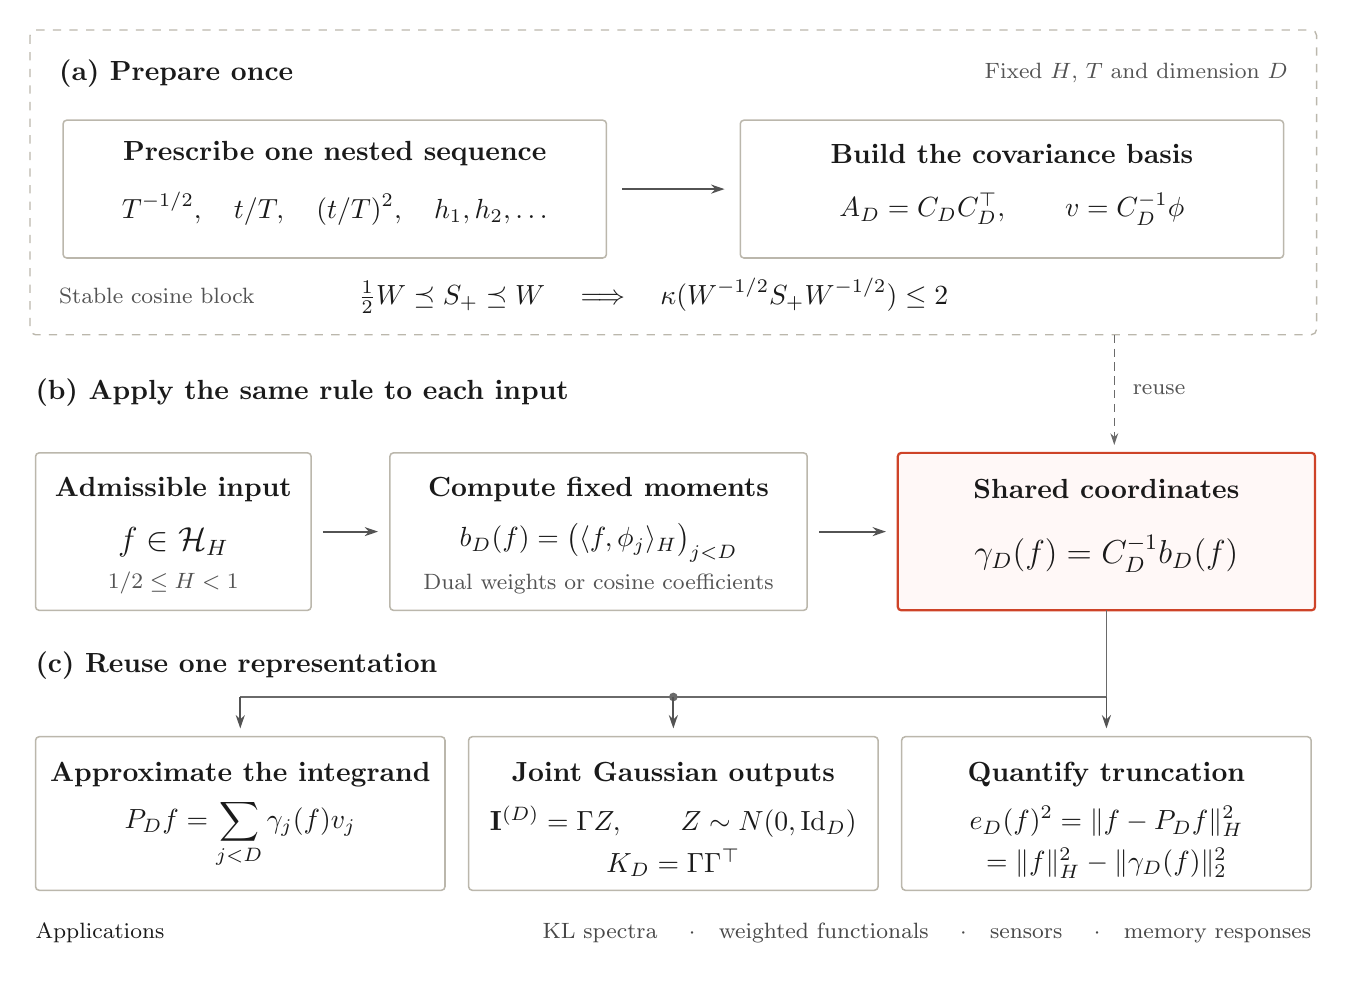
\begin{tikzpicture}[x=1mm,y=-1mm,font=\plotfont]
\path[use as bounding box] (0,0) rectangle (164,118);
% Preparation is fixed before any integrand is seen.
\draw[draw=soft!85!ink,line width=.5pt,dashed,rounded corners=2pt] (.3,.3) rectangle (163.7,39.0);
\node[anchor=west,font=\headfont] at (4,5.8) {(a) Prepare once};
\node[anchor=east,label] at (160,5.8) {Fixed $H$, $T$ and dimension $D$};
\node[card,minimum width=69mm,minimum height=17.5mm] (raw) at (39,20.5) {};
\node[font=\headfont] at (39,16.0) {Prescribe one nested sequence};
\node[font=\mathfont] at (39,23.0)
 {$\displaystyle T^{-1/2},\quad t/T,\quad (t/T)^2,\quad h_1,h_2,\ldots$};
\node[card,minimum width=69mm,minimum height=17.5mm] (basis) at (125,20.5) {};
\node[font=\headfont] at (125,16.0) {Build the covariance basis};
\node[font=\mathfont] at (125,23.0) {$A_D=C_DC_D^\top,\qquad v=C_D^{-1}\phi$};
\draw[flow] (75.5,20.5) -- (88.5,20.5);
\node[anchor=west,label] at (4,34.1) {Stable cosine block};
\node[anchor=west,font=\mathfont] at (42,34.1)
 {$\displaystyle \tfrac12 W\preceq S_+\preceq W
 \quad\Longrightarrow\quad \kappa(W^{-1/2}S_+W^{-1/2})\le2$};
% The repeated input rule has a single direction.
\node[anchor=west,font=\headfont] at (1,46.4) {(b) Apply the same rule to each input};
\draw[dependency] (138,39.0) -- (138,53);
\node[anchor=west,label,fill=white,inner sep=1pt] at (140,46) {reuse};
\node[card,minimum width=35mm,minimum height=20mm] (input) at (18.5,64) {};
\node[font=\headfont] at (18.5,58.6) {Admissible input};
\node[font=\fontsize{12}{14}\selectfont] at (18.5,65.3) {$f\in\HH$};
\node[label] at (18.5,70.5) {$1/2\le H<1$};
\node[card,minimum width=53mm,minimum height=20mm] (moments) at (72.5,64) {};
\node[font=\headfont] at (72.5,58.6) {Compute fixed moments};
\node[font=\mathfont] at (72.5,65.4) {$b_D(f)=\bigl(\langle f,\phi_j\rangle_H\bigr)_{j<D}$};
\node[label] at (72.5,70.7) {Dual weights or cosine coefficients};
\node[card,draw=coral!75!brown,fill=coral!4,minimum width=53mm,minimum height=20mm,line width=.8pt] (coords) at (137,64) {};
\node[font=\headfont] at (137,58.6) {Shared coordinates};
\node[font=\fontsize{12}{14}\selectfont] at (137,66.8) {$\gamma_D(f)=C_D^{-1}b_D(f)$};
\draw[flow] (37.5,64) -- (44.5,64);
\draw[flow] (100.5,64) -- (109,64);
% One coordinate representation serves all downstream calculations.
\node[anchor=west,font=\headfont] at (1,81.0) {(c) Reuse one representation};
\draw[draw=ink!65,line width=.6pt] (137,74) -- (137,85) -- (27,85);
\fill[ink!65] (82,85) circle[radius=.55mm];
\foreach \x in {27,82,137} \draw[flow] (\x,85) -- (\x,89);
\node[card,minimum width=52mm,minimum height=19.5mm] (approx) at (27,99.8) {};
\node[card,minimum width=52mm,minimum height=19.5mm] (joint) at (82,99.8) {};
\node[card,minimum width=52mm,minimum height=19.5mm] (tail) at (137,99.8) {};
\node[font=\headfont] at (27,94.9) {Approximate the integrand};
\node[font=\mathfont] at (27,102.4) {$\displaystyle P_Df=\sum_{j<D}\gamma_j(f)v_j$};
\node[font=\headfont] at (82,94.9) {Joint Gaussian outputs};
\node[font=\mathfont] at (82,100.8) {$\mathbf I^{(D)}=\Gamma Z,\qquad Z\sim N(0,\mathrm{Id}_D)$};
\node[font=\mathfont] at (82,106.1) {$K_D=\Gamma\Gamma^\top$};
\node[font=\headfont] at (137,94.9) {Quantify truncation};
\node[font=\mathfont] at (137,100.8) {$\displaystyle e_D(f)^2=\|f-P_Df\|_H^2$};
\node[font=\mathfont] at (137,106.1) {$=\|f\|_H^2-\|\gamma_D(f)\|_2^2$};
\node[anchor=west,font=\smallfont] at (1,115.0) {Applications};
\node[anchor=east,font=\smallfont,text=ink!80] at (163,115.0)
 {KL spectra \quad$\cdot$\quad weighted functionals \quad$\cdot$\quad sensors \quad$\cdot$\quad memory responses};
\end{tikzpicture}
\end{document}
